\section{Related work}

Over the last couple of years an increasing interest in reducing the inference time of intelligent applications to extend to real-time applications...

\subsection{Model optimization} 

Architectural: MobileNet, ShuffleNet

Compression: \cite{courbariaux_binaryconnect:_2015}

\subsection{Model Partitioning}

Neurosurgeon \cite{kang_neurosurgeon:_2017} is a lightweight partitioning scheduler, that uses knowledge of the individual layers of the \gls{dnn} to effectively reduce inference latency. Splitting a model to run on both cloud for Edge-Device mode is an inherent nature of sequential \gls{dnn}s, that at any layer can be stopped. The intermediate output are transferred over the network and continued at the next layer on an edge server, as shown in figure \ref{fig:offlaoding}.

\begin{figure}
	\centering
	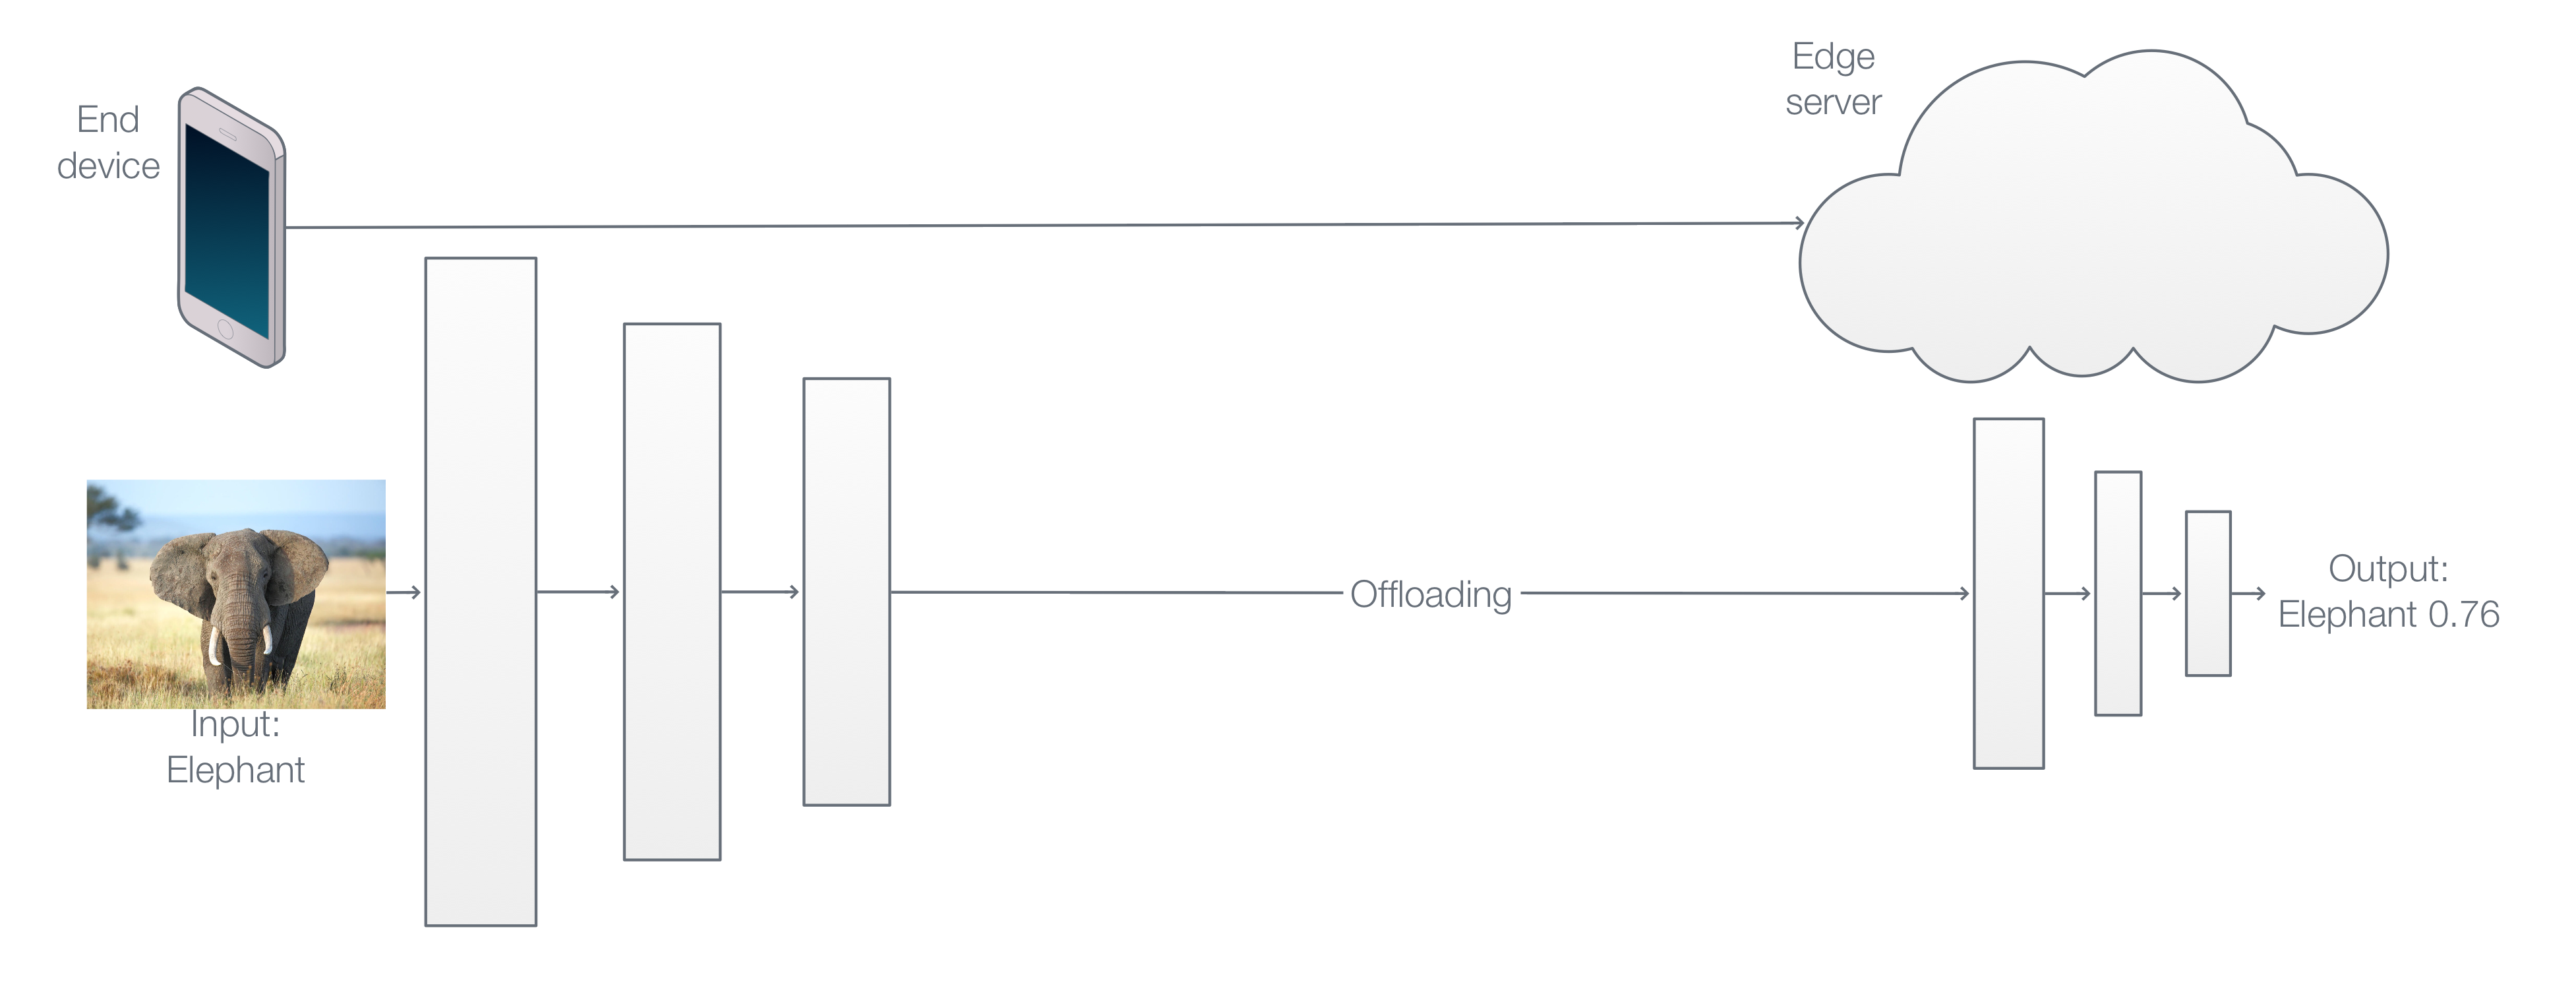
\includegraphics[width=\linewidth]{figures/models/offloading}
	\caption[Model partitioning]{Edge-Device model partitioning run part of the model on-device and offload the rest to edge processing. Network partitioning utilize the assumption, that at some later point in the \gls{dnn} a smaller representation of the data is found, illustrated by the gradually decreasing model layers, to reduce the communication bottleneck. }
	\label{fig:offlaoding}
\end{figure}

Communication latency is the bottleneck in an offloading application, hence a smaller representation of the input data is needed, however the layers producing a smaller output than the original input typically lies deep within the network. Neurosurgeon construct regression models for layer execution time and  output data size of the layers of a \gls{dnn}, to decide the best partition of the \gls{dnn} based on networking condition. The work is based on \gls{mcc} and shows, that the conventional cloud-only approach is insufficient due to different networking technologies and mobile device is becoming \gls{gpu} enabled. 
% Evidently moving computation to the edge reduces the communication latency. 

Another effort to reduce communication overhead of network splitting is adding feature compression of intermediate features before offloading to cloud \cite{choi_deep_2018}. The paper shows, that lossless compression have no impact on accuracy, however bit saving is rather limited. Lossy compression, on the other hand, results in 70\% bit savings, however also affects accuracy and require compression-aware training to compensate. The follow up paper \cite{choi_near-lossless_2018} propose compression techniques for deep features and achieve significant better bit saving, than conventional image compression algorithms. 

\gls{bottlenet} \cite{eshratifar_bottlenet:_2019} is a novel neural network module. Client-side it consists of a reduction unit and a compressor unit and server-side of a decompressor unit and restoration unit. The reduction unit creates a smaller representation of intermediate result by applying spatial- and channel-wise convolution. The compressor uses lossy \gls{jpeg} compression, that are decompressed server-side. The restoration unit apply deconvolution to restore the intermediate feature back to the required dimensionality for the next layer in the network. \gls{bottlenet} is able to achieve 84$\times$ bit savings compared to cloud-only approach with less than 2\% degradation of accuracy caused by lossy compression with compression-aware training. Under good networking condition, the evaluation of \gls{bottlenet} shows, that the best split is after the first convolutional block, as a smaller representation of the input can be found already here. Compared to cloud-only approach using WiFi a 8$\times$ speed up is found.

The collaborative scheme between end device and edge servers shows improvements for \gls{cpu}-enabled end devices, compared to a cloud-only approach, however as communication is introduced the overall latency will vary depending on the networking conditions. Model selection is an approach, that tries to limit the amount of offloading, by first running an on-device model. 

\subsection{Model Selection}

To obtain faster inference Big/Little \gls{dnn} \cite{park_big/little_2015} is simple approach using model selection. It implements a hybrid edge architecture of device-only and selective offloading for edge-only processing. It runs a smaller yet less accurate model on device and a larger more accurate model on the edge server, as illustrated by figure \ref{fig:big/little-dnn}. 

\begin{figure}
	\centering
	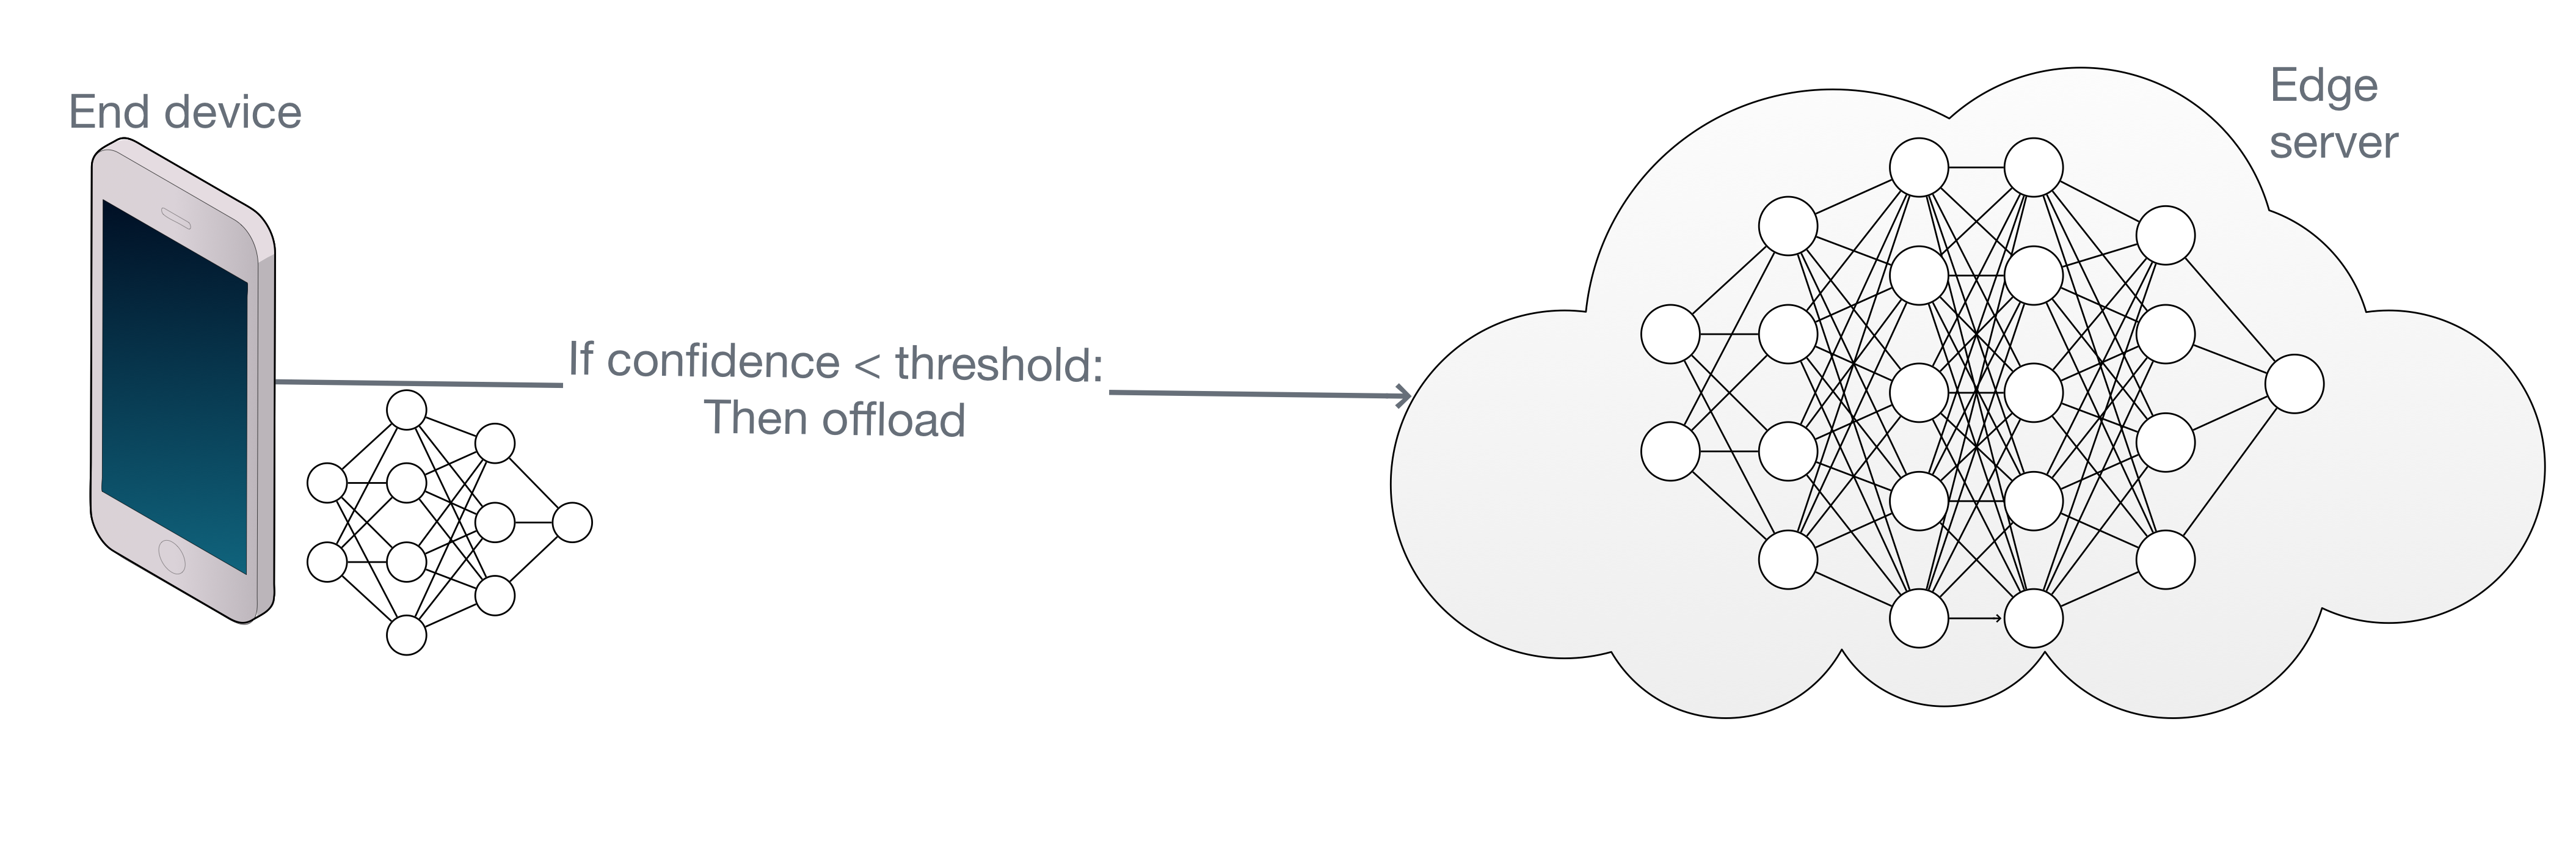
\includegraphics[width=.5\linewidth]{figures/models/big_little_dnn}
	\caption[Big/Little \gls{dnn} architecture]{Big/Little \gls{dnn}, a hybrid edge architecture. An on-device model is used to selectively offload to a more complex model hosted on an edge server.}
	\label{fig:big/little-dnn}
\end{figure}

If the prediction confidence of the little model is unsatisfactory, a decision is made to offload to the big model on the edge server. If a lot of samples are able to be correctly classified locally a speed-up is gained. However, the down-side of this approach is, if too many samples require the big model to satisfy a certain confidence threshold, a lot of work is wasted on the on-device prediction. Nonetheless the paper \cite{park_big/little_2015} contribute with another method to define a threshold, called \textsc{Score margin}. They have found, that the difference between the highest scoring and second highest scoring prediction, have a close relation to the actual true label. Although Big/Little \gls{dnn} obtain good results on energy savings and inference latency, more sophisticated frameworks such as early exiting, that also enabled model partitioning have been proposed.

\subsection{Model Early Exit}

\gls{branchynet} \cite{teerapittayanon_branchynet:_2016} proposed by \citeauthor{teerapittayanon_branchynet:_2016} is an early exiting framework for fast inference of a \gls{dnn}. The work states, that typically samples can be accurately classified using less \gls{dnn} layers which can improve the inference time, if a sample cannot be classified with proper confidence more layers can be used to obtain a more confident prediction. The framework shows promising results of reduced inference time, added regularization via joint optimization of exiting points and mitigation of vanishing gradients. The result are based on three well-known \gls{dnn} architectures; LeNet \cite{lecun_lecun-98.pdf_1998}, AlexNet \cite{krizhevsky_imagenet_2017} and ResNet \cite{he_deep_2015}, modified to implement the \gls{branchynet} framework, and to accommodate the MNIST \cite{lecun_mnist_2010} and Cifar-10 \cite{krizhevsky_cifar-10_nodate} datasets.  

\gls{ddnn} \cite{teerapittayanon_distributed_2017} also proposed by \citeauthor{teerapittayanon_distributed_2017}, extend upon \gls{branchynet} framework and show, that the architecture is suited for network partitioning. They propose a distributed computing hierarchy over cloud, edge and end devices. The work shows benefits from distributed computing to provide fault tolerance when end devices are failing. and I should mention other stuff... However \gls{ddnn} focuses on a cluster of end devices collaboratively solving a classification challenge, \gls{branchynet} on the other hand is more suited for \gls{p2p} applications and adaptively fit aforementioned \gls{ei} architectures, including device-only, edge-only and the collaborative edge-device architecture by network partitioning.


Using early exiting where a smaller representation of input data is obtained, thus less data must be offloaded to the edge server

\gls{msdnet} \cite{huang_multi-scale_2017} is a novel \gls{dnn} architecture specifically designed for early exiting. It extend upon the DenseNet \cite{huang_densely_2016} architecture, which they show to be more suitable for early exiting than the poputlar ResNet architecture, because of its unique densely connected blocks, which uses features from earlier layers for final classification. The combination of very general and increasingly more specific and complex feature are shown to be important for early exiting models. \gls{msdnet} uses the densely connected layers along with multi-scale path to further improve early layers accuracy, thus promoting early exiting.